En la siguiente sección se podrá observar una breve descripción del modelo de datos a usar. Los autores han decidido usar una base de datos orientada a grafos, Neo4j, por lo cual cada explicación se hará a grandes rasgos sobre un grafo ejemplo generado directamente en Neo4j.

Otro dato a tener en cuenta será que los autores \textbf{sólo describirán el modelo de datos que se ajusta, según ellos, a las funcionalidades a ser implementadas}.

En el capítulo \ref{chap:anexos} el lector podrá encontrar en detalle la descripción de cada nodo etiqueta.

\section{Modelo de datos de gestión de eventos}

Para el prototipo, se ha realizado solamente un evento de practica deportiva (de caracter libre). El modelo generado se puede apreciar en la figura \ref{fig:modelo_datos_gestion_eventos}.

\begin{figure}[!htb]
  \begin{center}
    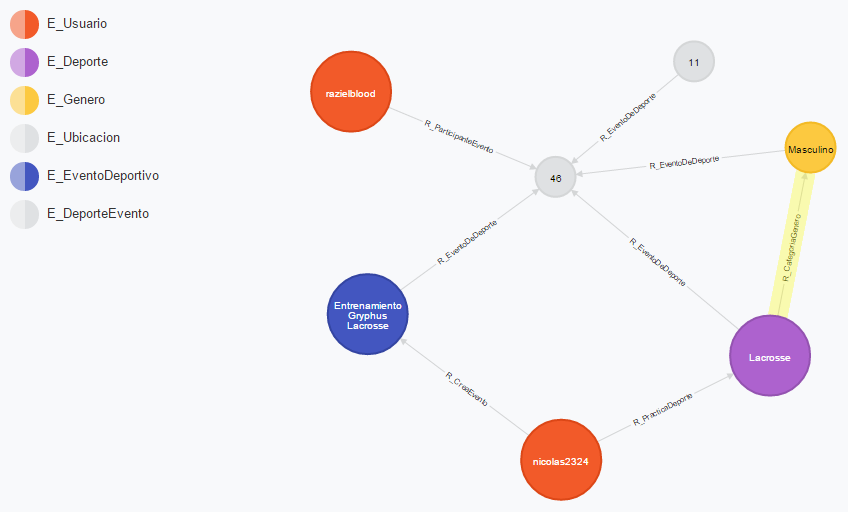
\includegraphics[width=11cm]{./imagenes/Modelo_de_datos/Gestion_eventos.png}
    \caption{Modelo de datos de gestión de eventos}
    \label{fig:modelo_datos_gestion_eventos}
    \textbf{Fuente:}  Autores
  \end{center}
\end{figure}

Sobre ésta parte del modelo de datos cabe aclarar el papel de E_DeporteEvento: Se utilizó un nodo cabecera E_EventoDeportivo para registrar características generales de un evento; E_DeporteEvento guarda detalles de ''eventos dentro del evento'', con tal de que en un evento de práctica deportiva quepa la posibilidad de incluir más de un deporte.

Los nodos que hacen referencia a relaciones n-arias son mostrados en gris.

\section{Modelo de datos de gestión de ubicaciones}

Sobre éste modelo de datos se puede encontrar ubicaciones espaciales atadas a los deportes registrados en la red social. El modelo generado se puede apreciar en la figura \ref{fig:modelo_datos_gestion_ubicaciones}.

\begin{figure}[!htb]
  \begin{center}
    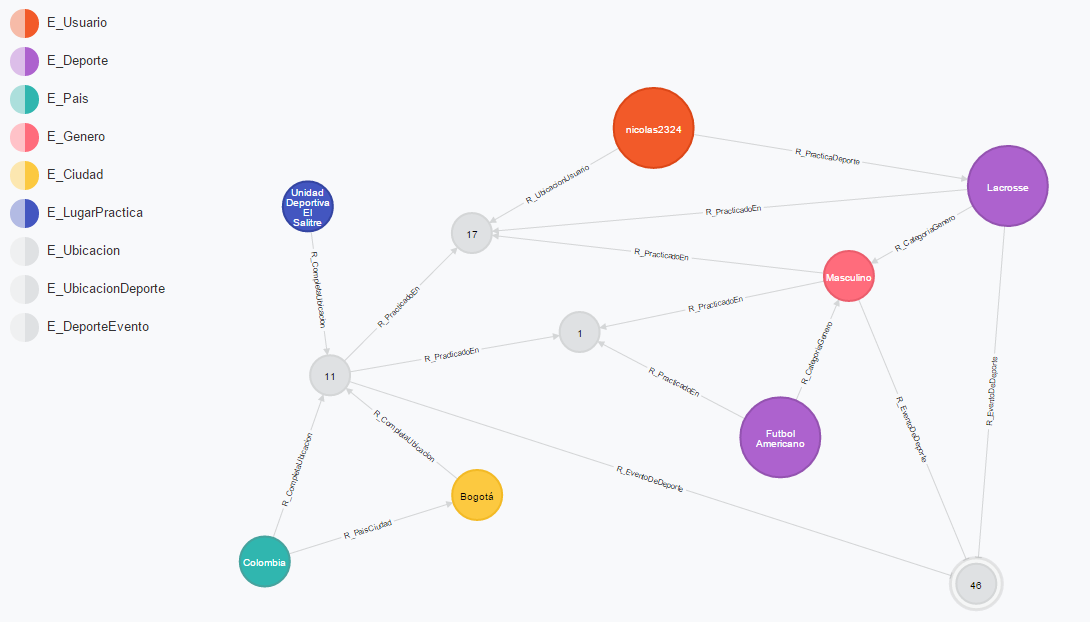
\includegraphics[width=11cm]{./imagenes/Modelo_de_datos/Gestion_ubicaciones.png}
    \caption{Modelo de datos de gestión de ubicaciones}
    \label{fig:modelo_datos_gestion_ubicaciones}
    \textbf{Fuente:}  Autores
  \end{center}
\end{figure}

Es debido observar los nodos que hacen referencia a relaciones n-arias: uno de ellos se ha llamado E_UbicacionDeporte, el cual tiene la función de ubicar a un deporte, atado a un respectivo género, en un lugar de práctica; E_Ubicacion hace un nodo referencia a todos los aspectos de ubicación que tiene una ubicación registrada en la red social, para éste caso, serán los países, ciudades y lugares exactos de práctica del deporte.

Los nodos que hacen referencia a relaciones n-arias son mostrados en gris.

\section{Modelo de datos de gestión de deportes}

Sobre éste modelo de datos se puede apreciar todas las características que los autores han querido atar (para el prototipo) a una entidad deporte, mostrando también su relación con el usuario. La relación con los eventos es debida verla en la figura \ref{fig:modelo_datos_gestion_eventos}, así como la relación en las ubicaciones es debida verla en la figura \ref{fig:modelo_datos_gestion_ubicaciones}. El modelo generado se puede apreciar en la figura \ref{fig:modelo_datos_gestion_deportes}.

\begin{figure}[!htb]
  \begin{center}
    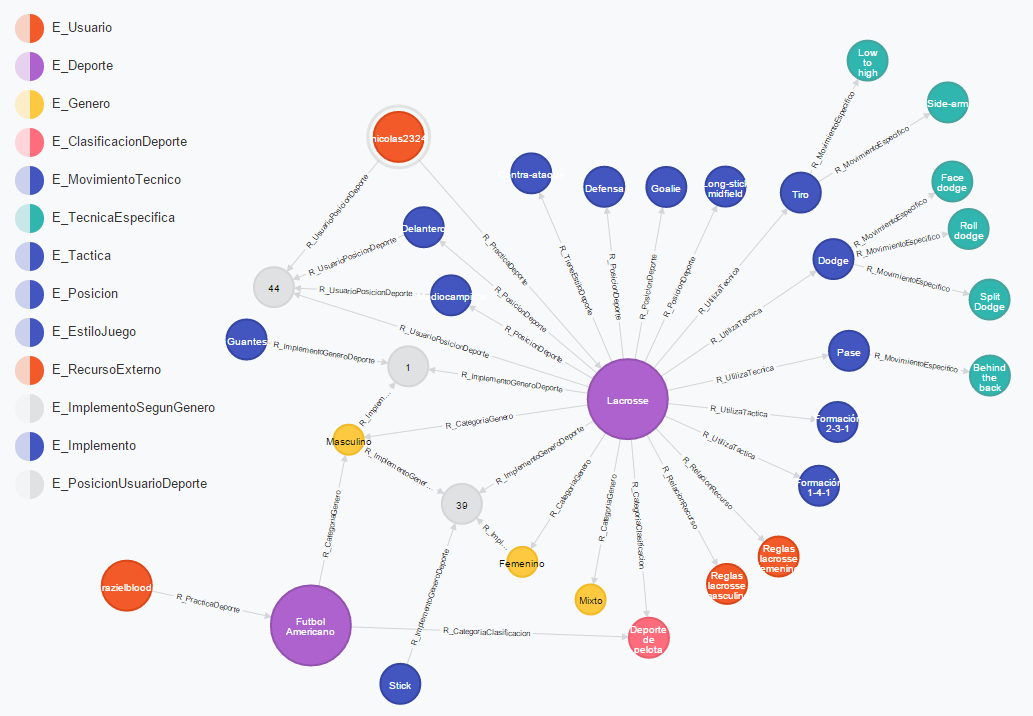
\includegraphics[width=11cm]{./imagenes/Modelo_de_datos/Gestion_deportes.png}
    \caption{Modelo de datos de gestión de deportes}
    \label{fig:modelo_datos_gestion_deportes}
    \textbf{Fuente:}  Autores
  \end{center}
\end{figure}

Sobre ésta parte del modelo se puede observar cómo todos los elementos que han incluido los autores son elementos unidos como nodos al deporte elegido. Hay dos relaciones n-arias que merecen ser explicadas: E_ImplementoSegunGenero es un nodo que actúa como relación n-aria entre E_Genero, E_Deporte y E_Genero, debido a que el equipamiento de un deporte puede variar entre género (por ejemplo, en el lacrosse las mujeres no utilizan guantes protectores); E_PosicionUsuarioDeporte es un nodo que funciona como relación n-aria entre E_Deporte, E_Usuario y E_Posicion, buscando comunicar en que posiciones juega generalmente un usuario para determinado deporte (en éste caso, el usuario \textit{nicolas2324} juega \textit{lacrosse}en las posiciones \textit{mediocampista} y \textit{delantero}).

Los nodos que hacen referencia a relaciones n-arias son mostrados en gris.